\newcommand{\svrname}{Mr Thomas Rees}
\newcommand{\jkfside}{oneside}
\newcommand{\jkfhanded}{right}

\newcommand{\studentname}{Harry Langford}
\newcommand{\studentemail}{hjel2@cam.ac.uk}

\documentclass[10pt,\jkfside,a4paper]{article}

\newcommand{\svcourse}{CST Part IA: Software Engineering and Security}
\newcommand{\svnumber}{1}
\newcommand{\svvenue}{Microsoft Teams}
\newcommand{\svdate}{2022-05-11}
\newcommand{\svtime}{15:00}
\newcommand{\svuploadkey}{CBd13xmL7PC1zqhNIoLdTiYUBnxZhzRAtJxv/ytRdM1r7qIfwMsxeVwM/pPcIo8l}

\newcommand{\svrname}{Dr Sam Ainsworth}
\newcommand{\jkfside}{oneside}
\newcommand{\jkfhanded}{yes}

\newcommand{\studentname}{Harry Langford}
\newcommand{\studentemail}{hjel2@cam.ac.uk}

% DO NOT add \usepackage commands here.  Place any custom commands
% into your SV work files.  Anything in the template directory is
% likely to be overwritten!

\usepackage{fancyhdr}

\usepackage{lastpage}       % ``n of m'' page numbering
\usepackage{lscape}         % Makes landscape easier

\usepackage{verbatim}       % Verbatim blocks
\usepackage{listings}       % Source code listings
\usepackage{epsfig}         % Embed encapsulated postscript
\usepackage{array}          % Array environment
\usepackage{qrcode}         % QR codes
\usepackage{enumitem}       % Required by Tom Johnson's exam question header

\usepackage{hhline}         % Horizontal lines in tables
\usepackage{siunitx}        % Correct spacing of units
\usepackage{amsmath}        % American Mathematical Society
\usepackage{amssymb}        % Maths symbols
\usepackage{amsthm}         % Theorems

\usepackage{ifthen}         % Conditional processing in tex

\usepackage[top=3cm,
            bottom=3cm,
            inner=2cm,
            outer=5cm]{geometry}

% PDF metadata + URL formatting
\usepackage[
            pdfauthor={\studentname},
            pdftitle={\svcourse, SV \svnumber},
            pdfsubject={},
            pdfkeywords={9d2547b00aba40b58fa0378774f72ee6},
            pdfproducer={},
            pdfcreator={},
            hidelinks]{hyperref}


% DO NOT add \usepackage commands here.  Place any custom commands
% into your SV work files.  Anything in the template directory is
% likely to be overwritten!

\usepackage{fancyhdr}

\usepackage{lastpage}       % ``n of m'' page numbering
\usepackage{lscape}         % Makes landscape easier

\usepackage{verbatim}       % Verbatim blocks
\usepackage{listings}       % Source code listings
\usepackage{graphicx}
\usepackage{float}
\usepackage{epsfig}         % Embed encapsulated postscript
\usepackage{array}          % Array environment
\usepackage{qrcode}         % QR codes
\usepackage{enumitem}       % Required by Tom Johnson's exam question header

\usepackage{hhline}         % Horizontal lines in tables
\usepackage{siunitx}        % Correct spacing of units
\usepackage{amsmath}        % American Mathematical Society
\usepackage{amssymb}        % Maths symbols
\usepackage{amsthm}         % Theorems

\usepackage{ifthen}         % Conditional processing in tex

\usepackage[top=3cm,
            bottom=3cm,
            inner=2cm,
            outer=5cm]{geometry}

% PDF metadata + URL formatting
\usepackage[
            pdfauthor={\studentname},
            pdftitle={\svcourse, SV \svnumber},
            pdfsubject={},
            pdfkeywords={9d2547b00aba40b58fa0378774f72ee6},
            pdfproducer={},
            pdfcreator={},
            hidelinks]{hyperref}

\renewcommand{\headrulewidth}{0.4pt}
\renewcommand{\footrulewidth}{0.4pt}
\fancyheadoffset[LO,LE,RO,RE]{0pt}
\fancyfootoffset[LO,LE,RO,RE]{0pt}
\pagestyle{fancy}
\fancyhead{}
\fancyhead[LO,RE]{{\bfseries \studentname}\\\studentemail}
\fancyhead[RO,LE]{{\bfseries \svcourse, SV~\svnumber}\\\svdate\ \svtime, \svvenue}
\fancyfoot{}
\fancyfoot[LO,RE]{For: \svrname}
\fancyfoot[RO,LE]{\today\hspace{1cm}\thepage\ / \pageref{LastPage}}
\fancyfoot[C]{\qrcode[height=0.8cm]{\svuploadkey}}
\setlength{\headheight}{22.55pt}


\ifthenelse{\equal{\jkfside}{oneside}}{

 \ifthenelse{\equal{\jkfhanded}{left}}{
  % 1. Left-handed marker, one-sided printing or e-marking, use oneside and...
  \evensidemargin=\oddsidemargin
  \oddsidemargin=73pt
  \setlength{\marginparwidth}{111pt}
  \setlength{\marginparsep}{-\marginparsep}
  \addtolength{\marginparsep}{-\textwidth}
  \addtolength{\marginparsep}{-\marginparwidth}
 }{
  % 2. Right-handed marker, one-sided printing or e-marking, use oneside.
  \setlength{\marginparwidth}{111pt}
 }

}{
 % 3. Alternating margins, two-sided printing, use twoside.
}


\setlength{\parindent}{0em}
\addtolength{\parskip}{1ex}

% Exam question headings, labels and sensible layout (courtesy of Tom Johnson)
\setlist{parsep=\parskip, listparindent=\parindent}
\newcommand{\examhead}[3]{\section{#1 Paper #2 Question #3}}
\newenvironment{examquestion}[3]{
\examhead{#1}{#2}{#3}\setlist[enumerate, 1]{label=(\alph*)}\setlist[enumerate, 2]{label=(\roman*)}
\marginpar{\href{https://www.cl.cam.ac.uk/teaching/exams/pastpapers/y#1p#2q#3.pdf}{\qrcode{https://www.cl.cam.ac.uk/teaching/exams/pastpapers/y#1p#2q#3.pdf}}}
\marginpar{\footnotesize \href{https://www.cl.cam.ac.uk/teaching/exams/pastpapers/y#1p#2q#3.pdf}{https://www.cl.cam.ac.uk/\\teaching/exams/pastpapers/\\y#1p#2q#3.pdf}}
}{}


\usepackage{graphicx}
\graphicspath{ {./images/} }
\usepackage{enumitem}
\usepackage{amsmath}

\begin{document}

\begin{enumerate}[label=(\alph*)]

\item 

\begin{examquestion}{2015}{4}{3}

Consider the transformations used in the construction and rendering of a three 
dimensional model on a screen.

\begin{enumerate}[label=(\alph*)]

\item List the three principal transformations used in the processing pipeline and 
explain their roles.

\begin{itemize}

\item Translation

To move the position of objects in the scene. This can be simply to change the location -- ie make 
an object sit on a plane or to move it to the right -- or to place a given object either fully or 
partially behind another object. Having translations in matrices applied to multiple instances of one 
object can move them to differeent places and make them distinct.

\item Scaling

To change the size of objects in the scene. This makes objects smaller or larger and enables the 
same base object to be used for different things (ie you can start off with a single instance of a 
cube, duplicate and resize them and then the cubes can be used completely differently).

\item Rotation

To change the orientation of objects in the scene. Perhaps to attach an object to another or simply to 
make the scene look better.

\end{itemize}

\item Why is it convenient to represent the transformations as matrices?

You can combine multiple operations together by multiplying matrices together. 
This means that complicated series of transformations can be pre-calculated 
and then applied to a large number of points without recalculatiion 
-- and since the matrices are precalculated and do not need to be changed during 
rendering, the multiplication can be performed in parallel. This is very efficient.

Matrices provide a standard format for storage and transformations. Without them 
there is no easy way to represent transformations, rotations and scalings in the 
same format. Matrices also standardise transformations across dimensions -- there is 
no constraint on the dimensionality of a matrix or the transformations which it can 
be applied to. This means that 2D transformations, 3D transformations and beyond can 
be standardised.

Matrices are a simple comcept to visualise and understand. Understanding how transformations 
work makes it much easier to actually apply them.

GPU's are optimised for matrix multiplication. This means that performing transformations using 
matrices results in faster rendering than other methods.

\item What are homogeneous coordinates? Explain how they are used in modelling 
these transformations as matrices.

Homogeneous coordinates are 4-dimensional coordinates $(x', y', z', w)$ where 
$w$ is a scaling factor. This ``scaling'' factor allows transformations to be 
expressed as a matrix without preventing translations and scalings.

Homogenous coordinates allow for $\Theta(1)$ time scalings (provided that 
you are scaling all the coordinates by the same amount) -- since you can 
divide the value of $w$ by a scaling factor and that will scale the coordinates 
by the same scaling factor.

The conversion from homogeneous coordinates $(x', y', z', w)$ to 3D coordinates 
$(x, y, z)$ is $x = \frac{x'}{w}$, $y = \frac{y'}{w}$ and $z=\frac{z'}{w}$.
The conversion takes $\Theta(1)$ time -- however since matrix multiplication is 
$\Theta(n^3)$ (na\"ively) with respect to the dimensionality of a square $n\times n$ matrix, 
this means that matrix multiplication with homogeneous coordinates 
takes approximately twice as long as with standard 3D coordinates. This is generally 
more efficient, since matrix transformations are calculated once and then applied to 
many hundreds or thousands of coordinates. It is far more efficient to take the 
overhead associated with adding an extra dimension in the matrices than to apply 
for example $M_0$, $T_0$, $M_1$, $T_1$, $M_2$ to 1000 different points (where $M_i$ 
is a matrix and $T_i$ is a translation).

\item Derive the matrix to represent a perspective transformation for  a viewer at 
the origin of a point in three dimensions to a point on a screen in the plane $z = d$.

This transformation will require a translation. Translations in matrices require the 
operations to be done in homogeneous coordinates. The general 3D coordinates of a 
point on the plane $z = d$ are $(x_0, y_0, d)$. The matrix to do this translation 
is given below:

$\begin{pmatrix}
1 & 0 & 0 & x_0\\
0 & 1 & 0 & y_0\\
0 & 0 & 1 & d\\
0 & 0 & 0 & 1\\
\end{pmatrix}$

\end{enumerate}

\end{examquestion}

\item

\begin{examquestion}{2010}{4}{4}

\begin{enumerate}[label=(\alph*)]

\item Homogeneous coordinates are often used to represent transformations in 3D:

\begin{center}
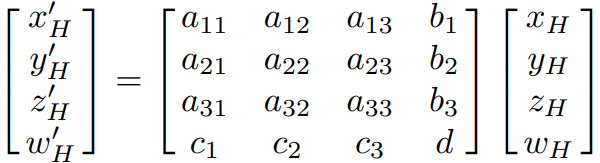
\includegraphics[scale=0.5]{homocords}
\end{center}

\begin{enumerate}[label=(\roman*)]

\item Explain how to convert standard 3D coordinates, $(x, y, z)$, to 
homogeneous coordinates, and how to convert homogeneous coordinates to 
standard 3D coordinates.

To convert standard 3D coordinates $(x, y, z)$ to homogeneous coordinates 
$(x', y', z', w)$, create an arbitrary (non-zero) variable $w$ (often initially 1 for convenience). 
Then define $x' = w\cdot x$, $y' = w\cdot y$ and $z' = w\cdot z$.

To convert homogeneous coordinates $(x', y', z', w)$ to standard 3D coordinates $(x, y, z)$, 
define $x = \frac{x'}{w}$, $y = \frac{y'}{w}$ and $z = \frac{z'}{w}$.

\item Describe the types of transformations provided by each of the four blocks 
of coefficients in the matrix $(a_{11}\dots a_{33}\ b_{1}\dots b_{3}, c_1\dots c_3\text{ and } d)$.

$a$'s provide rotations and scaling (when the scaling factor for $x$, $y$, $z$ is different), $b$'s provide 
translations, $c$'s provide scalings dependant where the scaling factor is dependant on $(x,y,z)$ and $d$ provides 
a universal constant scaling factor -- ie if you want to scale everything by 2 then you can multiply $w$ by 
$\frac{1}{2}$.

\begin{itemize}
\item a's do rotations and scalings. b's do translations, d does scalings too (but only if you scale 
all the components by the same amount. c does some sort of scaling dependant on xyz.
\end{itemize}

\item Explain what transformation is produced by each of the following matrices:

\begin{center}
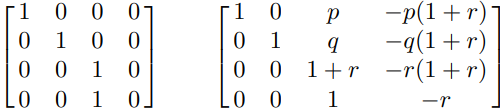
\includegraphics[scale=0.7]{matrixtransforms}
\end{center}

The left matrix scales the coordinates $(x, y, z)$ by a factor of $\frac{1}{z}$ changing them to 
$(\frac{x}{z}, \frac{y}{z}, 1)$.

Let the right matrix be notated by $M$.

\begin{equation}
\begin{split}
M &= \begin{pmatrix}
1 & 0 & p & -p\cdot(1 + r)\\
0 & 1 & q & -q\cdot(1 + r)\\
0 & 0 & 1 + r & -r\cdot(1 + r)\\
0 & 0 & 1 & -r\\
\end{pmatrix}\\
&= \begin{pmatrix}
1 & 0 & 0 & 0\\
0 & 1 & 0 & 0\\
0 & 0 & 1 & 0\\
0 & 0 & \frac{1}{1 + r} & 0\\
\end{pmatrix} \cdot
\begin{pmatrix}
1 & 0 & p 	  & -p\cdot(1 + r)\\
0 & 1 & q 	  & -q\cdot(1 + r)\\
0 & 0 & 1 + r & -r\cdot(1 + r)\\
0 & 0 & 0 	  & 1\\
\end{pmatrix}\\
&= \begin{pmatrix}
1 & 0 & 0 & 0\\
0 & 1 & 0 & 0\\
0 & 0 & 1 & 0\\
0 & 0 & \frac{1}{1 + r} & 0\\
\end{pmatrix} \cdot
\begin{pmatrix}
1 & 0 & p & 0\\
0 & 1 & q & 0\\
0 & 0 & 1 + r & 0\\
0 & 0 & 0 & 1\\
\end{pmatrix}\cdot
\begin{pmatrix}
1 & 0 & 0 	  & -p\\
0 & 1 & 0	  & -q\\
0 & 0 & 1	  & -r\\
0 & 0 & 0 	  & 1\\
\end{pmatrix}\\
\end{split}
\end{equation}

So the matrix $M$ is equal to a scaling of the $z$ coordinate of $\frac{1}{1+r}$. Let $z' = \frac{1}{1+r}$.
Then a shear parallel to the $z$ axis. Call these new coordinates $(x'', y'', z'')$. 
$z'' = \frac{(1+r)\cdot z}{1+r} = z$. Then there is a translation of $(-p, -q, -r)$.
So the matrix $M$ represents a scaling proportional to $\frac{1}{1+r}$, then a shear parallel to the $z$ axis and 
a translation.

\end{enumerate}

\item Consider the following figure:

\begin{center}
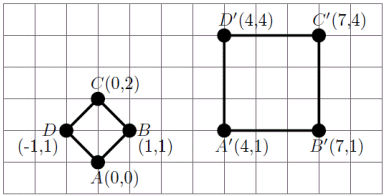
\includegraphics{gridwsquares}
\end{center}

\begin{enumerate}[label=(\roman*)]

\item Give a matrix, or product of matrices, that will transform the square $ABCD$ 
into the rectangle $A'B'C'D'$.

To transform the square $ABCD$ into $A'B'C'D'$, we first have to rotate it $\frac{\pi}{4}^c$ clockwise, 
then scale it by a factor of $\frac{3}{\sqrt{2}}$ and translate it by $(4, 1)$.
Since this sequence involves a translation, to have a single matrix to represent this transformation we must 
use homogeneous coordinates and adding a variable $w$.

Let $T$ be the resultant transformation.

\begin{equation}
\begin{split}
T &=
\begin{pmatrix}
\frac{\sqrt{2}}{2} & \frac{\sqrt{2}}{2} & 0\\
-\frac{\sqrt{2}}{2} & \frac{\sqrt{2}}{2} & 0\\
0 & 0 & 1\\
\end{pmatrix}
\cdot 
\begin{pmatrix}
1 & 0 & 0\\
0 & 1 & 0\\
0 & 0 & \frac{\sqrt{2}}{3}\\
\end{pmatrix}
\cdot
\begin{pmatrix}
1 & 0 & 4\\
0 & 1 & 1\\
0 & 0 & 1\\
\end{pmatrix}\\
T &= 
\begin{pmatrix}
\frac{\sqrt{2}}{2} & \frac{\sqrt{2}}{2} & 0\\
-\frac{\sqrt{2}}{2} & \frac{\sqrt{2}}{2} & 0\\
0 & 0 & \frac{\sqrt{2}}{3}\\
\end{pmatrix}
\cdot
\begin{pmatrix}
1 & 0 & 4\\
1 & 1 & 1\\
0 & 0 & 1\\
\end{pmatrix}\\
T &= 
\begin{pmatrix}
\frac{\sqrt{2}}{2} & \frac{\sqrt{2}}{2} & 4\cdot\frac{\sqrt{2}}{3}\\
-\frac{\sqrt{2}}{2} & \frac{\sqrt{2}}{2} & \frac{\sqrt{2}}{3}\\
0 & 0 & \frac{\sqrt{2}}{3}\\
\end{pmatrix}
\end{split}
\end{equation}

\item Show what happens if the same transformation is applied to $A'B'C'D'$.

If we apply the same transformation to $A'B'C'D'$, we do not get the desired 
transformation since our original transformation rotates and scales around the origin 
-- and $A'B'C'D'$ is not at the origin.

Applying the matrix transformation $T$ to $A'B'C'D'$ gives the coordinates: 
$A'' = (11.5, -3.5)$, $B'' = (16, -8)$, $C'' = (20.5, -3.5)$ and $D'' = (16, 1)$

\end{enumerate} 

\end{enumerate}

\end{examquestion}

\item Explain what a MIPmap is, how to create one, why one would want to use one, where one 
would be used, and how one is used.

A MIPmap is a way of storing a texture map where you store $k$ levels of resolution of the image -- 
with the $0^\text{th}$ level being the normal resolution and the $(k + 1)^\text{th}$ level 
having a quarter the resolution of the $k^\text{th}$ level. This allows very quick and 
accurate downsampling (since the results have essentially been precomputed). It also only 
takes a third more space that the normal texture map.

Downsampling must happen when the resolution of the texture map for an object at a point is greater 
than the resolution of the point that the texture map is for. This can either happen at 
the edge of a shape when the surface is almost parallel 
to the view vector $\^v$ or when the texture map is a far higher resolution than the shape it is 
being mapped onto. In the first case, there are often only a few pixels which need to be downsampled. 
Although it can be incredibly innefficient to do this (downsampling by a factor of 10 requires sampling 
10 pixels with conventional methods -- but only two pixels with a MIPmap [technically 1 but more likely 2]), 
often in the first situation there are not many pixels which have to be downsampled and so this is tolerable. 
However, in the second situation, every pixel on the object's surface must be downsampled. This means that it 
takes 10x longer to render the objects texture. Using a MIPmap means that it will only require 2 samples and 
so is 5x faster in this situation.

You downsample on a MIPmap by finding the value $k = \log_2D$ where D is the width of the pixel to be 
downsampled (where the pixel is not square any reasonable method can be taken to estimate it's width -- 
say the arithmetic mean or geometric mean of the sides -- or simply the longest side). Then linearly 
interpolate the texture between the $\lfloor k\rfloor^\text{th}$ and $\lceil k\rceil^\text{th}$ level 
of the MIPmap. A quicker (but less accurate) approximation to this would be to take a single sample 
from the nearest level.

\end{enumerate}

\end{document}

